The methods, in general, performed alright.  
However, as stated earlier, the optimal parameters for 2018 turned out to be different from those for 2017.  
For instance, in the 2017 data, the optimal parameters were:\newline\newline
\begin{tabular}{|c|l|}
\hline
Classifier & Parameters \\
\hline
LR & $C=1e-8$ \\
SVM & ker=sigmoid \\
RF & $max\_dep=5$, $num\_est=40$ \\
\hline
\end{tabular} \newline\newline
While the reasons for this disparity are not explored here, it raises the question of whether this year was anomalous, or if every year you can expect different parameters to perform better.  
The actual evaluation of this, however, is a bit beyond the current purposes of this project.  
As such, the following results are from using the optimum parameters on the 2018 dataset.  
The RF classifier, due to the random nature of the classifier performs differently every time it is run.  
Rarely, it does better than every other classifier.  
Also rarely, it does far worse.  
On average, it seems to perform about on par with the PageRank classifier.  
The LR classifier consistently scores the best (with the exception of the RF classifier on few select occasions) with $850$ points.  
The SVM classifier came just above that, with $860$ points.  
Third was the standard PageRank algorithm with $620$ points, followed closely by the RF classifier with a total of $600$ points.    
In the basement are the GNB ($510$ points) and MYC ($360$ points) classifiers.  
\begin{figure}
\centering
\caption{Total Score Through Time : The cumulative score for each algorithm after every round has been finished.}
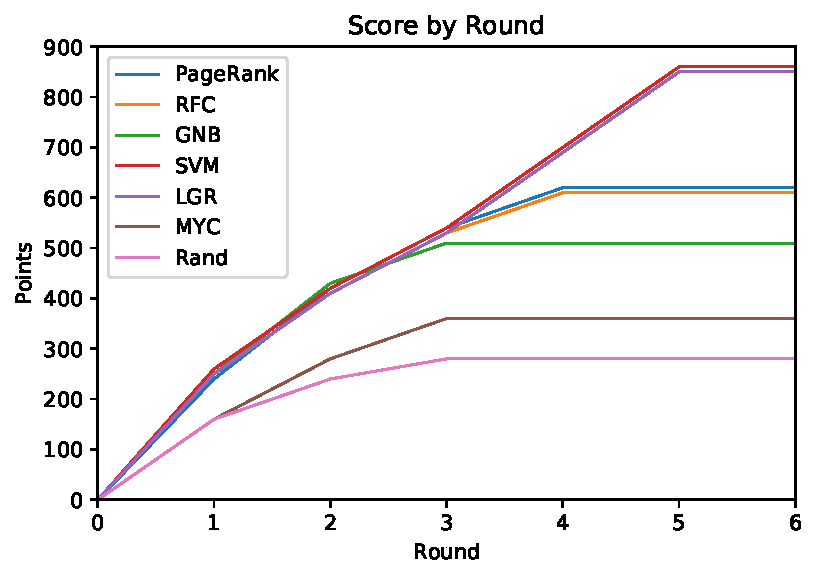
\includegraphics[width=0.5\textwidth]{../Current_Scores.pdf}
\label{fig:scores1}
\end{figure}
The cumulative scores, by round, are displayed in Figure \ref{fig:scores1}.  
The random line shows the expected score from randomly guessing, as opposed to any one random bracket.  
For reference, the following table contains which team each classifier predicted to win the entire tournament, and when that team was eliminated.\newline\newline
\begin{tabular}{|c|c|c|}
\hline \\
Class. & Champion & Round Eliminated \\
\hline \\
PgRnk & Duke & Elite 8 \\
RFC & UNC & R 32 \\
GNB & Duke & Elite 8 \\
SVM & Virginia & R 64 \\
LGR & Virginia & R 64  \\
MYC & Duke & Elite 8 \\
\hline
\end{tabular}
